\section{一对多对应关系编码与端到端网络}\label{symnet_方法}

\par 本节系统阐述基于一对多对应关系与对称感知的6D物体位姿估计方法。该方法旨在突破传统一对一对应方法在对称模糊性问题上的局限性,通过将传统二进制编码方案(已在单目对应方法中验证有效性\cite{2024hipose, su2022zebrapose})拓展至一对多对应编码,构建对称感知的编码方式。经过网络端到端学习后,该编码可直接解码生成最终位姿预测结果,无需依赖RANSAC算法及基于渲染的后处理流程。

\par 对于给定具有已知内参的RGB图像和一组物体的CAD模型,目标是估计图像中每个物体相对于相机的姿态(旋转矩阵 $\bm{R} \in SO(3)$ 和平移向量 $\bm{t} \in \mathbb{R}^3$)。注意,对于非对称物体,只有一个真实标注位姿 $\bm{T}=[\bm{R}|\bm{t}]$,而对于对称物体,则有多个可能的真实标注位姿 $\bm{T}_k, k=1, 2,...,n$,其中 $n$ 是真实标注位姿的数量,可以是无限的。

\par 在接下来的部分中,详细比较了一对一对应关系和一对多对应关系。随后,介绍了估计6D物体位姿的方法,包括从表面编码到最终位姿估计的整个过程。

\subsection{一对一对应关系}

提取一对一对应关系是对应关系方法中的关键组成部分,它表示从观测图像中的2D点 $\bm{p}_i=(u_i,v_i)$ 和物体模型中的3D点 $\bm{P}_j=(x_j,y_j,z_j)$ 之间的匹配,记为 $\bm{o}_r = (\bm{p}_i, \bm{P}_j)$,其中 $\bm{p}_i\in \mathbb{R}^2$ 和 $\bm{P}_j\in \mathbb{R}^3$。对应关系可以基于逐点的真实位姿 $\bm{T}$ 得出:

\begin{equation}
        \bm{p}_i=\pi(\bm{T} \bm{P}_j) 
        \label{eq:projection}
\end{equation}

其中 $\pi(\cdot)$ 是使用内参矩阵的针孔相机模型的投影函数,其中成像畸变已根据标定参数进行校正。定义一对一对应关系集 $\bm{O} = \{\bm{o}_1, \bm{o}_2, ..., \bm{o}_m\}$,包含 $m$ 个一对一对应关系,其中 $\bm{o}_r = (\bm{p}_i, \bm{P}_j)$。透视n点(PnP)算法的目标是根据一组给定的一对一对应关系来计算位姿 $\bm{T}$。主流基于对应关系的位姿估计方法普遍依赖一对一对应关系作为辅助学习信号。在非对称物体场景下,此类对应虽能唯一确定物体位姿,但在处理对称物体时则存在固有歧义性,导致位姿估计结果不唯一。

对于对称物体的每个真实位姿 $\bm{T}_k$,可以使用\autoref{eq:projection} 获得一对一对应关系集。然而,在训练阶段,将具有显著不同对应关系集的相似图像设置为学习目标可能会导致收敛问题。

在\autoref{fig:one_one_corres} 中展示了立方体和圆柱体的不同一对一对应关系集。第一列:无纹理的立方体和圆柱体图像。第一行:立方体图像的三种可能的对应关系集。第二行:圆柱体图像的三种可能的对应关系集。右三列中模型的颜色表示物体局部坐标系中的坐标,红色、绿色和蓝色分别表示 x 轴、y 轴和 z 轴的坐标。物体局部坐标系由彩色箭头表示。虚线显示了2D-3D对应关系。在训练过程中,上述不同的对应关系都可能作为输入图像的辅助变量,相当于网络需要学习相同输入但是不同输出的结果。

\begin{figure}[htbp]
    \centering
    \begin{overpic}[width=0.75\textwidth]{figure/symnet/one-to_one-correspondence.jpg}
        \put(4,2){物体图像}
        \put(43,2){多种一对一对应关系}
    \end{overpic}
    \caption{对称物体的多种一对一对应关系}
    \label{fig:one_one_corres}
\end{figure}

\subsection{一对多对应关系} 

2D点 $\bm{p}_i=(u_i,v_i)$ 和所有可能的3D点集合 $\bm{Y}_j = \{\bm{P}_{j,1}, \bm{P}_{j,2}, ..., \bm{P}_{j,n}\}$ 之间的匹配定义为一对多对应关系,记为 $\bm{o}_r = (\bm{p}_i, \bm{Y}_j)$。一对多对应关系应满足以下条件:

\begin{equation}
\bm{p}_i = \pi(\bm{T}_k  \bm{P}_{j,k}), \quad k = 1,2,...,n
\label{eq:projection_one_to_many}
\end{equation}

\par $\bm{T}_k$ 是所有可能的真值位姿。
定义了一对多对应关系集 $\bm{O}_\text{sym} = \{\bm{o}_1, \bm{o}_2, ..., \bm{o}_m\}$,包含 $m$ 个一对多对应关系,其中 $\bm{o}_r = (\bm{p}_i, \bm{Y}_j)$。
\autoref{fig:many_many_corres}展示了立方体和圆柱体的一对多对应关系。图中用相同的颜色纹理表示3D点属于相同的一对多对应关系。\autoref{fig:many_many_corres}左图假设立方体只有沿z轴旋转0度、90度、180度和270度的4种对称性,蓝色线条和绿色线条分别展示了角和侧面中心的两组一对多对应关系。不可见部分用虚线,可见部分用实线。\autoref{fig:many_many_corres}右图:展示了圆柱体的一对多对应关系,其中侧面和顶部表面的两个特定一对多对应关系用线条表示。

\par 一对多对应关系表明,从一个像素 $\bm{p}_i$ 出发,不可能确定匹配的3D点坐标 $\bm{P}_j$,但可以确定对应的3D点集 $\bm{Y}_j$。与一对一对应关系相比,一对多对应关系由于其无歧义性,为网络提供了一个更容易学习的任务。

\begin{figure}[ht]
\centerline{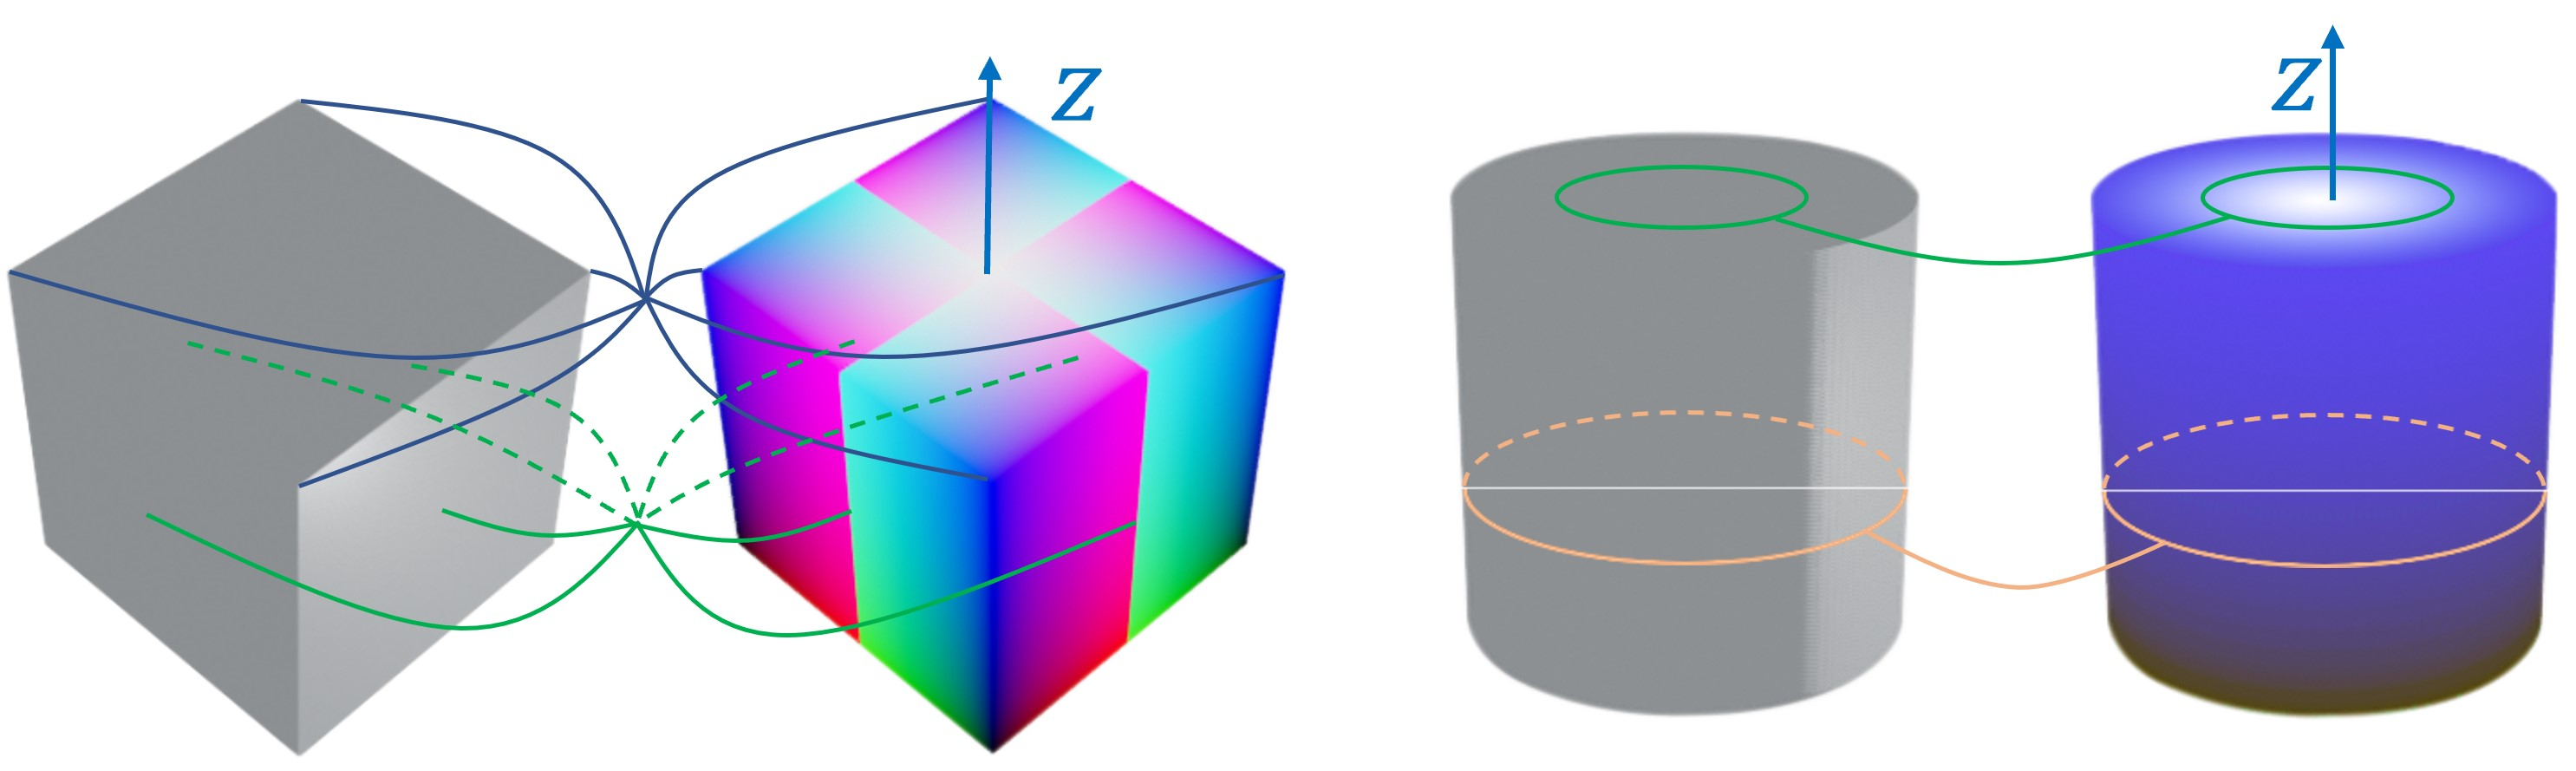
\includegraphics[width=0.75\textwidth]{figure/symnet/one-to-many-correspondence.jpg}}
\caption{对称物体一对多对应关系}
\label{fig:many_many_corres}
\end{figure}

\subsection{考虑对称的表面编码}

\par 采用离散二进制编码 $\bm{c}_r$ 对每个一对多对应关系 $\bm{o}_r$ 进行编码。如 \autoref{fig:SymCode生成过程} 所示,该编码生成流程包含多个阶段:(a) 输入原始CAD模型作为处理基底;(b) 针对复杂拓扑结构进行人工部件划分以提升精度;(c) 基于对称优先级分类顶点对称类型;(d) 针对连续对称与离散对称特性分别建立主顶点索引机制;(e) 采用唯一性二进制编码策略,基于顶点几何特征生成对应编码$\bm{c}_i$;(f) 表面编码器基于二进制编码机制对模型顶点实施对称感知编码;(g) 将生成的编码标签作为网络中间监督信号。其中虚线框标注的预处理步骤可根据实际需求灵活配置。

\begin{figure}[htbp]
    \centering
    \begin{overpic}[width=1.0\textwidth]{figure/symnet/process_of_model.jpg}
        \put(7,51){模型}
        \put(28,51){模型分区}
        \put(53,51){对称性测试}
        \put(79,51){对称性映射}
        \put(10,24){渲染标签}
        \put(40,24){表面编码}
        \put(70,24){迭代编码生成}
    \end{overpic}
    \caption{SymCode生成过程和标签渲染}
    \label{fig:SymCode生成过程}
\end{figure}

\textbf{一对多对应关系生成原理 } 对于具有对称属性的物体,存在多个刚体变换操作能够将某一真实标注位姿 $\bm{T}_1$ 映射到其对称等效位姿 $\bm{T}_k$。具体而言,定义满足该条件的刚体运动集合为:

\begin{equation}
\bm{M} = \{\bm{m}\in SE(3)\ |\ \bm{T}_1  \bm{m} \in \{\bm{T}_1, \bm{T}_2,..., \bm{T}_n\} \}
\label{eq:rigid_motions}
\end{equation}
其中 $\bm{T}_1$ 表示任意一个真实标签位姿,$\bm{T}_k$ 表示其对称等效位姿,$n$ 为对称变换作用下可能存在的等效位姿总数。该集合 $\bm{M}$ 完整描述了物体对称性所允许的所有刚体运动可能性。

\textbf{对称性分类与主顶点 } 物体对称性可划分为两个基本类别:
1)离散对称性:其对应刚体变换集合 $\bm{M}$ 成离散群,包含可列个对称变换操作;
2)连续对称性:对应$\bm{M}$形成具有连续参数的李群结构。

\par 对于离散对称,给定顶点 $\bm{P}$ ,通过对称性生成其所有对称等效顶点集合:

\begin{equation}
\bm{P}_{j,k}=\bm{m} \bm{P},\quad k=1,2,..,n, \quad \bm{m} \in \bm{M}\label{eq:generate_correspondence}
\end{equation}

\par 注意,提供的模型表面上不一定存在对称等效顶点 $\bm{P}_{j,k}$。如果它们尚不存在,将把相应的顶点 $\bm{P}_{j,k}$ 添加到模型表面。此步骤确保模型中的每个顶点在一对多对应关系中都有其对应的对称等效顶点。随后,属于同一一对多对应关系的顶点将根据 \autoref{eq:generate_correspondence} 分为一组。

\par 对于连续对称,表面的顶点沿对称轴旋转变换实现集合参数化,最终在一个平面上对齐,如\autoref{fig:SymCode生成过程}(d)所示。通过这样做,旋转后在平面上同一位置的顶点被合并到同一个对应关系中。可以将旋转过程形式化如下:

\begin{equation}
\tilde{\bm{P}}=
\begin{bmatrix}
 \sqrt{x^2+y^2}  &0 &z
\end{bmatrix}^T
\label{eq:rotation_projection}
\end{equation}

这里,$\tilde{\bm{P}}$ 是原始顶点 $\bm{P}$ 的转换后的对称等效顶点。$x, y, z$ 分别表示 $\bm{P}$ 的三个分量。假设旋转发生在 z 轴上,结果平面是 x-y 平面,如\autoref{fig:SymCode生成过程}(d) 所示。所有能够转换成同一对称等效顶点的点被分为一组。

\textbf{复合对称性处理方法 } 对于T-LESS数据集\cite{tless},不同的物体仅标注了主要的对称类型。可以选择直接基于这种对称性注释生成一对多对应关系。然而,许多物体由多种对称类型的部分混合组成。考虑一个在立方体上方正放一个圆柱体组合而成的物体。虽然整个物体整体表现离散离散对称性,但在遮挡场景中使用基于离散对称性构建的对应关系仍会导致歧义。

此外,某些物体呈现“近似对称”特性,即其结构除部分小细节外整体对称。为应对这一挑战,开发了一种高级注释工具,能够提升物体模型标注的精确度。这是整个流程中唯一需要人工干预的环节,但操作简便,仅需几分钟即可完成。对于完全对称的物体,该步骤可省略,从而使整个注释流程实现完全自动化。该工具可以处理BOP\cite{hodan2024bop}提供的对称性注释格式的信息。

物体上的点可分为以下四类:(1) 无对称性,(2) 连续对称性,(3) 离散对称性,和 (4) n 重对称性。n 重对称性是离散对称性的一个特例,即对称角度为
\begin{equation}
\theta=i \cdot 2\pi /n,\quad i \in \{1,...,n\}
\end{equation}

如\autoref{fig:SymCode生成过程}(a) 提供了这种情况的示例。该物体的主体部分为绕轴线的旋转对称,模型上方的凸起无对称性。需要对物体存在的不同的对称类型的点进行分类。分类是通过每个顶点与应用\autoref{eq:generate_correspondence} 变换后的最近顶点之间的平均距离来确定的。由于不同类型的对称性本质上具有包含关系,连续对称性包含在离散对称性中,离散对称性包含在 n 重对称性中,而不属于上述任何类型的顶点将被视为无对称性。按以下顺序评估对称性:连续对称性、离散对称性、n 重对称性,最后是无对称性,称之为对称优先级。主要对称类型在数据集的元信息中提供。然而,对于破坏对称性的细节,需要人工干预来指定它们并确保识别出正确的对称类型。此外,还可以使用从经验或实验观察中得出的误差阈值来辅助识别对称类型 $sym$。对于给定的对称类型 $sym$,将基于该对称性生成对应关系集 $\bm{M}$ 并计算在此特定对称类型 $sym$ 下的误差如下:

\begin{equation}
\bm{e}_{j,sym} = \sum_{m\in\bm{M}}\left \|  \bm{P}_{\text{near}} - \bm{m}\bm{P} \right \| 
\end{equation}
其中 $\bm{P}_{\text{near}}$ 是指物体表面上与变换顶点 $\bm{m}\bm{P}$ 最近的顶点。

在移除属于高优先级对称性的顶点后,剩余的顶点可以分类到低优先级对称性类别中。任何未分类为任何对称性类型的顶点将被识别为无对称性。

为了获得更精确的分类,可以将模型细分为更小的区间,从而在每个区间内识别不同形式的潜在对称性。这种方法允许对对称结构进行更细致的分类,如\autoref{fig:SymCode生成过程}(b)所示。

\textbf{对应关系编码 } 已经建立了一对多对应关系集 $\bm{O}_\text{sym}$,其中每个组 $\bm{Y}_j$ 包含顶点 $\bm{P}_{j,k}$。此外,每个组 $\bm{Y}_j$ 都与一个对称类型 $sym$ 相关联。引入了一种对一对多对应关系集进行编码的方法。物体表面通过为一对多对应关系集引入分层二进制分组方案进行编码。

编码表示该像素匹配到的对应组 $\bm{Y}_j$。设计的编码应满足以下标准:1)为位姿估计提供足够的信息,对于具有不同对称类型的两个组 $\bm{Y}_j$ 和 $\bm{Y}_j'$,编码应表现出显著差异。2)为了便于网络学习,彼此接近的对应关系应具有更相似的编码。3)每个 $\bm{Y}_j$ 对应一个唯一的编码。
通常,从每个对应关系中选择一个3D顶点,称为主顶点,同时考虑邻近对应关系的空间接近性。主顶点将在下一步中用于实现二进制编码。

接下来,介绍如何为每组对应关系获取主顶点(prime point)。对于具有连续对称性的对应关系,使用\autoref{eq:rotation_projection} 将顶点映射到平面上,选择该顶点作为主顶点。对于其他类型的对称性,基于以下标准选择主顶点,该标准可以替换为其他满足条件(2)的方法。在该方法的实现中,所使用的标准计算每个对应关系中每个顶点的各坐标分量的绝对值之和。然后根据以下公式选择主顶点,记为 $\tilde{\bm{P}}$:
\begin{equation}
    \tilde{\bm{P}} = \max_{\bm{P}_{j,k}}
    (\left | x_{j,k} \right | +\left | y_{j,k} \right | +\left | z_{j,k} \right |), \quad \bm{P}_{j,k} \in \bm{Y}_j
\end{equation}

如\autoref{fig:SymCode生成过程}(e)所示,该物体的主顶点由彩色顶点表示。在对应关系中,只有一个顶点不是对称的,它将作为主顶点,颜色为绿色。
对于连续对称性,主顶点(红色)位于通过\autoref{eq:rotation_projection} 计算的平面上。
对于2重对称性,坐标值较高部分的顶点将作为主顶点,颜色为蓝色。

\textbf{迭代编码生成 } 迭代编码的灵感来自于一对一对应方法中使用的二进制编码\cite{su2022zebrapose}。ZebraPose\cite{su2022zebrapose} 构建了一个包含 $N$ 个物体模型顶点的二进制编码,定义了唯一对应于顶点 $\bm{P}_j$ 的 $d$ 位二进制编码 $\bm{c}_{j}$。二进制编码是通过迭代构建的,在每一步中将网格分成相等数量的顶点,并为每组分配一个位。在表面划分的第 $it$ 次迭代中,$it \in \{0, 1, \text{\textellipsis}, d-1\}$,有 $2^{it+1}$ 个独立的子组。给定一组顶点,划分是通过平衡的 k均值聚类(k-means)进行的,结果形成两个子组。对于非对称物体,一对多对应关系等同于一对一对应关系,因为没有由于对称性引起的歧义。

给定一对多对应关系集,希望用一个二进制编码 $\bm{c}_i \in {0, 1}^d$ 来表示每个对应关系 $\bm{o}_i$,其中 $d$ 是二进制编码的长度。基于每个对应关系的主顶点构建这样的编码。

在\autoref{fig:SymCode生成过程}(e)中,展示了执行 $d$ 次主顶点分组迭代的过程。分组迭代从所有主顶点的集合 $G$ 开始。对于具有二进制编码 $\bm{c}_i$ 的组 $G_{i}$,使用非平衡的k均值聚类(k-means)将其分成两组。结果组被分配编码 $\bm{c}_i \ll 1$ 和 $(\bm{c}_i \ll 1) + 1$,其中操作 $\ll$ 表示二进制左移。最终,获得 $2^d$ 个组,每个组都有其二进制编码。这些二进制编码可以用从 $0$ 到 $2^d - 1$ 的十进制形式表示。表面编码器如\autoref{fig:SymCode生成过程}(f)所示,其中颜色表示二进制编码 $\bm{c}_i$ 的十进制值,白色表示$2^d - 1$,黑色表示$0$,灰色为十进制数的线性映射颜色渐变。

\textbf{渲染 } 如\autoref{fig:SymCode生成过程}(f),对于标签位姿,能够渲染出唯一的渲染标签。渲染标签通过RGB格式进行存储,在使用过程中需要解码为16位的渲染标签作为辅助变量引导网络学习物体的真实位姿。如\autoref{fig:渲染与存储}中,最左侧图像为存储图像,右侧的图像为若干位解码后的渲染标签。

\begin{figure}[ht]
    \centerline{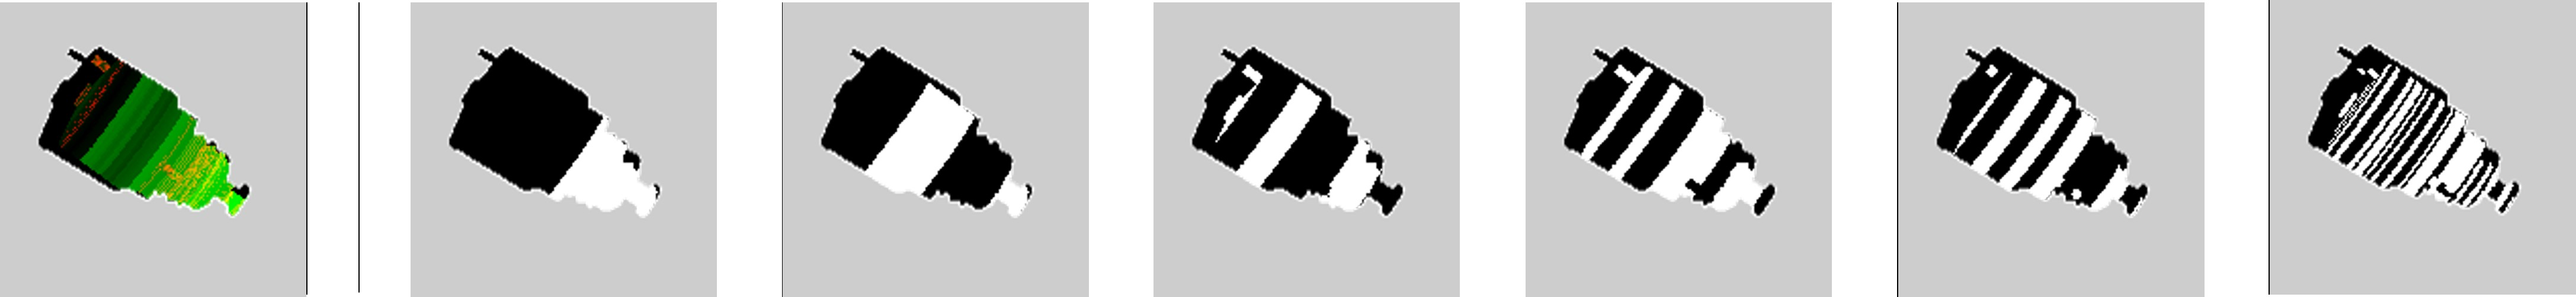
\includegraphics[width=1.0\textwidth]{figure/symnet/渲染与存储.jpg}}
    \caption{存储图与编码图}
    \label{fig:渲染与存储}
\end{figure}

\subsection{网络架构}
\begin{figure}[t]
    \centerline{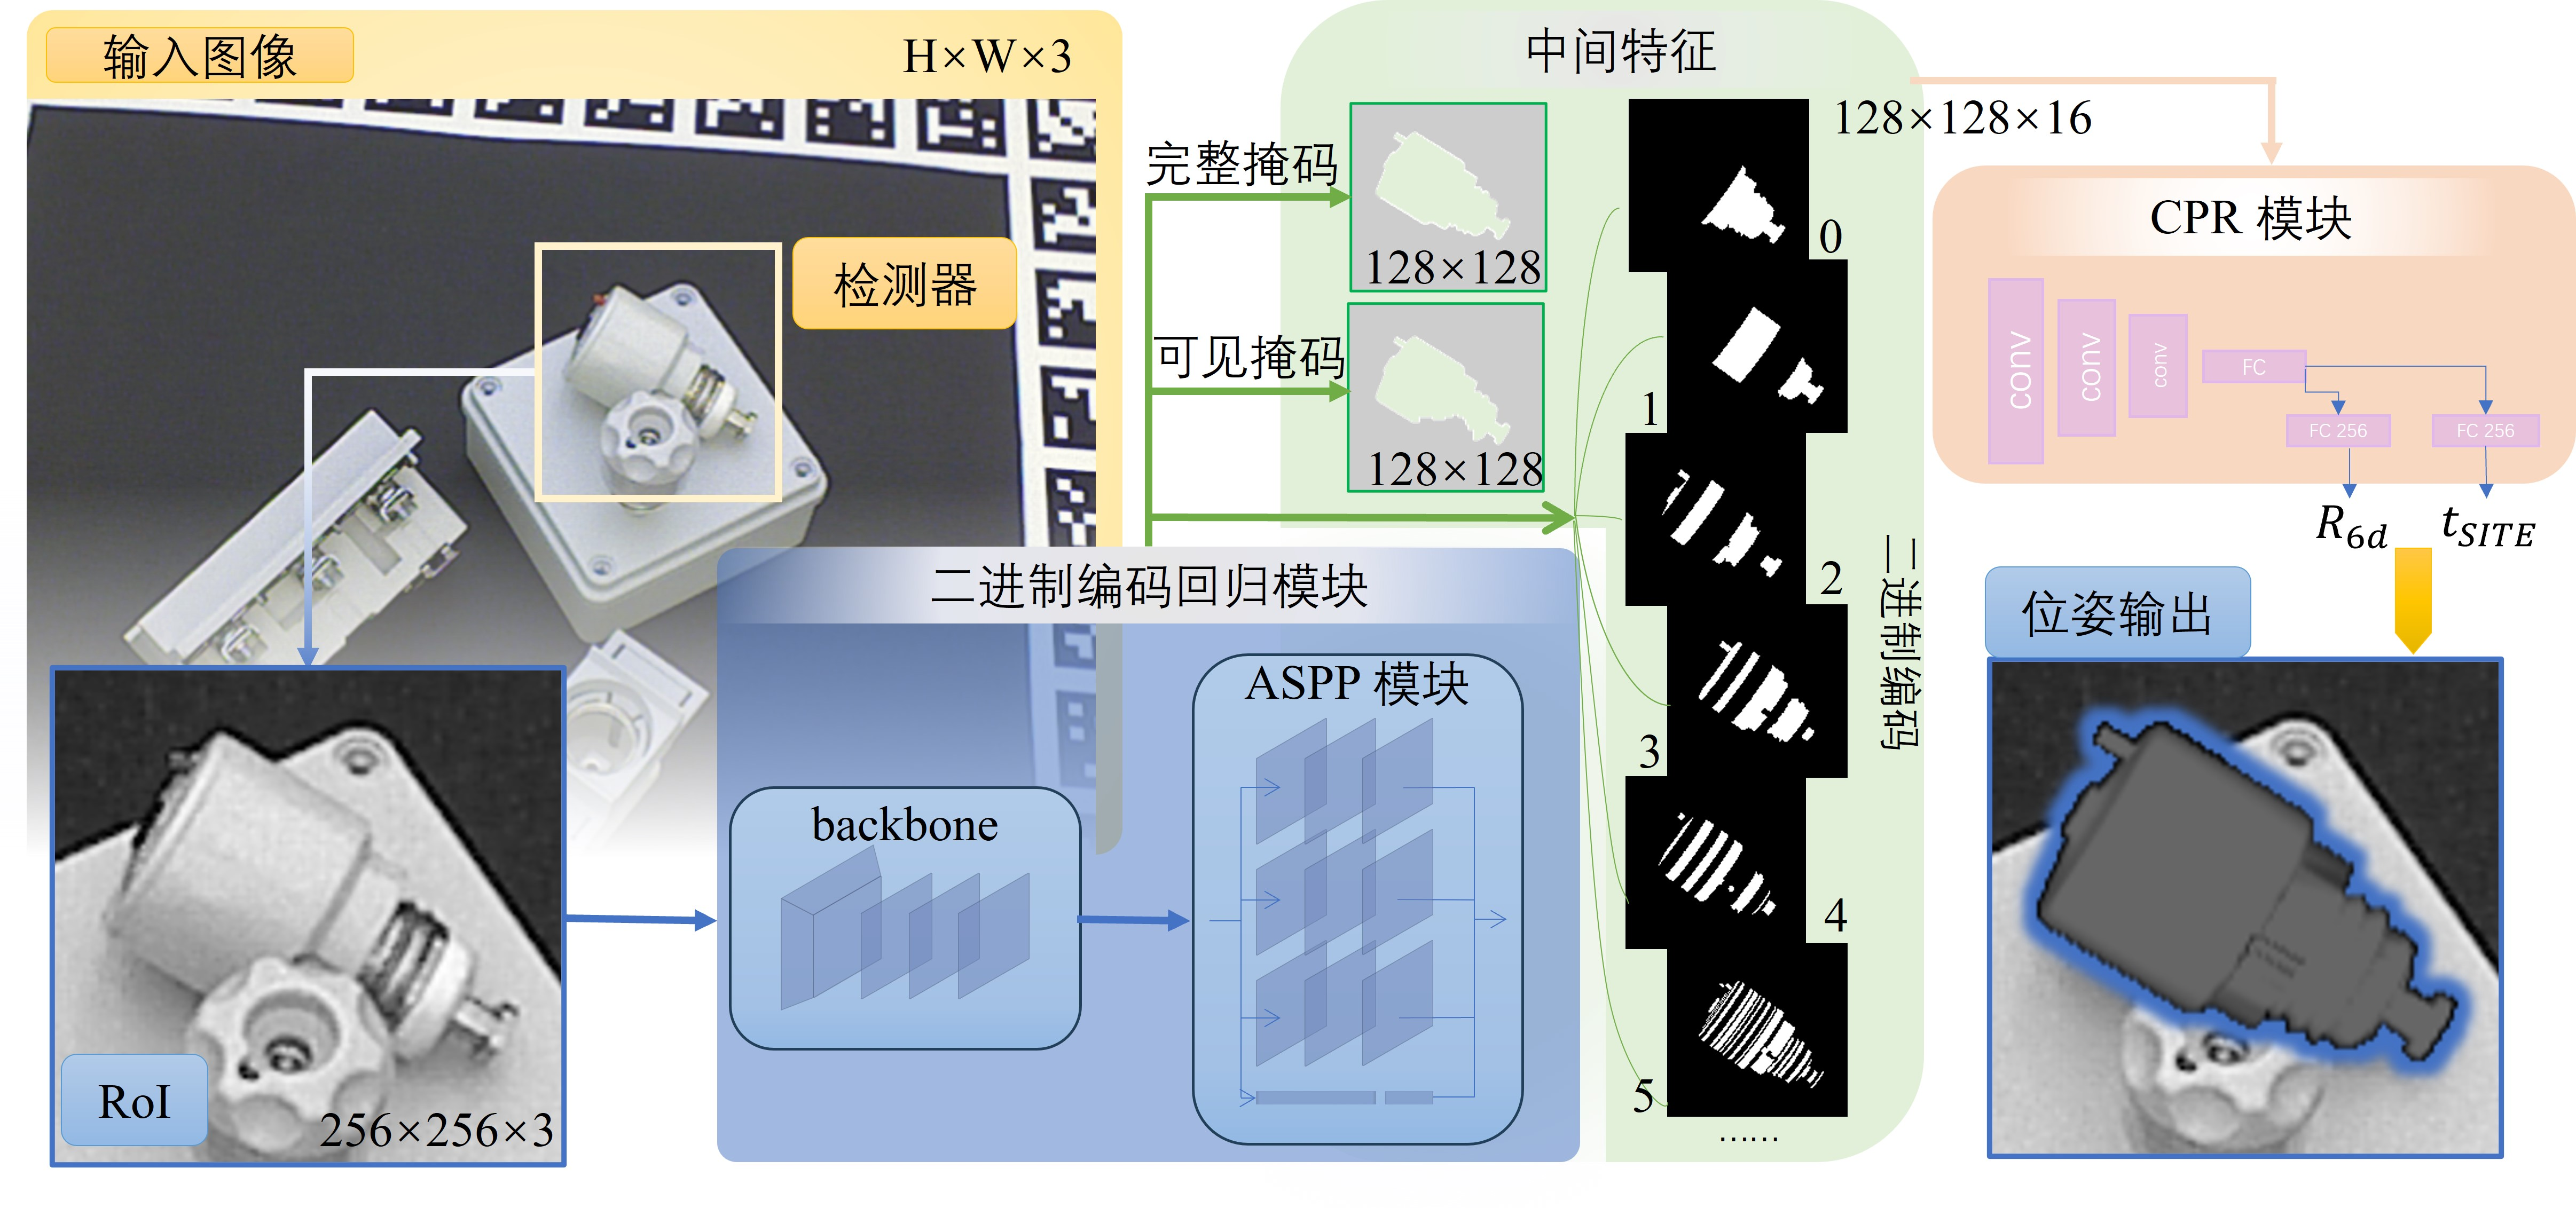
\includegraphics[width=1.0\textwidth]{figure/symnet/network.jpg}}
    \caption{SymNet框架}
    \label{fig:SymNet框架}
\end{figure}

本小节介绍SymNet框架。给定一张RGB图像,SymNet以放大的兴趣区域(RoI)作为输入,并预测包括掩码和二进制编码图在内的中间特征。然后,CPR模块直接回归6D物体位姿。整个过程是一个端到端的过程,消除了对PnP/RANSAC精调过程的需求。

在\autoref{fig:SymNet框架}中,通过检测器,找到物体的检测区域。通过对检测区域进行裁剪和分割,得到一个尺寸为$256 \times 256 \times 3$的RoI。RoI传入二进制编码模块,输出的中间变量包括尺寸为$128 \times 128$的物体完整掩码$M_{\text{amo}}$、尺寸为$128 \times 128$的可见掩码$M_\text{{vis}}$和尺寸为$128 \times 128 \times 16$的SymCode图。随后,这些中间变量被用作对应关系姿态回归(CPR)模块的输入。

二进制编码模块包括一个ResNet-34骨干网络\cite{he2016resnet},并利用了空洞空间金字塔池化(ASPP)\cite{chen2017deeplabv3},该方法在并行的空洞卷积中对特征进行不同尺度的重采样非常有效。我们还尝试了不同的卷积策略和来自CDPN\cite{li2019cdpn}的上采样方法作为网络架构的一部分,但结果没有显著差异。最终采用的网络细节见\autoref{fig:SymNet网络细节图}。

\begin{figure}[htbp]
    \centering
    \begin{overpic}[width=1.0\textwidth]{figure/symnet/具体网络细节图.jpg}
        \put(5,37){检测}
        \put(36,37){二进制编码模块}
        \put(85,37){CPR模块}
    \end{overpic}
    \caption{SymNet网络细节图}
    \label{fig:SymNet网络细节图}
\end{figure}

利用一个精炼的基于对应关系的位姿回归(CPR)模块,直接从可见掩码 $M_\text{{vis}}$、无模态掩码 $M_{\text{amo}}$ 和 SymCode 图 $M_\text{code}$ 回归6D位姿。CPR模块包括三个卷积层,每个卷积层后面跟着组归一化和ReLU激活。随后,两个全连接层应用于展平的特征。最后,两个并行的全连接层分别输出参数化为 $\bm{R}_{6d}$~\cite{zhou2019continuity} 的3D旋转和参数化为 $\bm{t}_\text{SITE}$~\cite{li2019cdpn} 的3D平移。网络的总参数量为 $63.2M$。

对可见掩码、无模态掩码和SymCode图使用$L1$损失。训练损失定义为
\begin{equation}
    Loss = L_\text{masks} + L_\text{code} + L_\text{params} + L_\text{ADD-S}
\end{equation}
$L_\text{params}$ 对应于端到端训练的损失,使用$L1$损失来处理 $\bm{R}_{6d}$ 和 $\bm{t}_\text{SITE}$。此外,$L_\text{ADD-S}$ 项源自PoseCNN的工作\cite{ycbv}:
\begin{equation}
L_\text{ADD-S} = \sum_{\bm{p} \in \bm{P}} \left\| \bm{R}_\text{gt} \cdot \bm{m} \bm{p} - \bm{R}_\text{pred} \bm{p} \right\|
\end{equation}
其中,
\begin{equation}
    \bm{m} = \mathop{\arg\min}\limits_{\bm{m} \in \bm{M}} \, re\left( \bm{R}_{\mathrm{gt}} \bm{m}, \bm{R}_{\mathrm{pred}} \right)
\end{equation}
这里 $re(\cdot, \cdot)$ 表示旋转角度误差的计算函数。

在训练过程中,所有损失同时进行训练,没有任何参数被冻结。在初步实验中,还探索了一种非端到端的训练策略,其中 $L_\text{masks} + L_\text{code}$ 用于训练二进制编码模块,而 $L_\text{params} + L_\text{ADD-S}$ 仅用于训练 CPR 模块;然而,这导致了结果的轻微下降。


\section{ZebraPoseSAT}

\par \autoref{symnet_方法}中介绍了一对一对应关系以及一对多对应关系,那么是否能够构造出基于一对一对应关系,但是没有对称歧义的方法呢?

\par 在ZebraPose\cite{su2022zebrapose}基础上实现ZebraPoseSAT(Symmetry-aware Training,SAT)。该方案通过解析方法\cite{pitteri2019object},在生成ZebraPose编码前,将所有真实位姿 $\bm{T}_i$ 基于Frobenius范数映射至唯一$\bm{T}$。作为BOP 2023挑战赛\cite{hodan2024bop}最佳纯RGB方法获奖方案,ZebraPoseSAT为SymNet提供了强有力的对比基准。

\par 在这个方案中,目的是保证同样输入的图片需要有唯一的标签,因此可以设计唯一性指标,从所有的对称性真值姿态$R_i$映射到同一真值姿态$R$。该映射关系可以用函数$f$进行表示:
\begin{equation}
    \bm{R} = f(\bm{R}_i) = \bm{R}_i \bm{m}, \quad \bm{m} = \arg\min_{\bm{m} \in \bm{M}} \|\bm{R}_i \bm{m} - \bm{I}\|
\end{equation}
不难发现,对于所有的$\bm{R}_i \bm{m}$都会映射为$\bm{R}$。\autoref{fig:zebraposesat}展现了一个连续对称物体的真值姿态转换过程。这个过程并不会影响$\bm{t}$。

\begin{figure}[htbp]
    \centering
    \begin{overpic}[width=0.7\textwidth]{figure/symnet/zebraposesat.pdf}
    \end{overpic}
    \caption{ZebraPoseSAT姿态映射}
    \label{fig:zebraposesat}
\end{figure}

\par 尽管该方法能够实现一对一映射,从而避免了位姿估计中的歧义问题,但其仍存在一个可能影响神经网络学习效果的潜在挑战:旋转参数的不连续性。具体而言,在网络从图像到位姿的推理过程中,某些旋转参数的变化会引入不连续现象。以绕轴180度的二重对称场景为例,当将$[180,360)$度区间的角度值映射至$[0,180)$区间时,真值为1度的图像仍保持1度的标签,而真值为359度的图像则被映射为179度。然而,真值为1度与真值为359度的图像在视觉上高度相似,但其对应的位姿参数却存在显著差异。这种不连续性要求神经网络能够有效区分视觉上极为接近的图像,并输出差异较大的位姿参数,从而增加了学习难度。尽管如此,实验结果表明,该方法在基础方案上仍实现了约$1\%$
的精度提升。
